\documentclass[10pt]{article}

\def\Type{LessonCaelan}
\def\TypeNum{Lesson 13}
\def\TypeTitle{Absolute Extreme Values\\Key }
\def\Semester{Fall 2021} %Not Used 
\def\Course{MATH 1190 \& 1210}
\def\Targets{  {\bf\color{RedOrange}A2} }

\usepackage{preambleDJ}
\usepackage{comment}
%\usepackage{ragged2e}


%%%%%%%%%%%% BEGIN DOCUMENT %%%%%%%%%%%%%%%
%%%%%%%%%%%% BEGIN DOCUMENT %%%%%%%%%%%%%%%
%%%%%%%%%%%% BEGIN DOCUMENT %%%%%%%%%%%%%%%
%%%%%%%%%%%% BEGIN DOCUMENT %%%%%%%%%%%%%%%
%%%%%%%%%%%% BEGIN DOCUMENT %%%%%%%%%%%%%%%




\begin{document}

\pagestyle{otherpages}
\thispagestyle{firstpage}
\vs{.5}

\textbf{Intended Learning Outcomes}
After this lesson, you will be able to 

\begin{itemize}
    \item Define absolute extrema and describes its difference from local extrema. (\target{A2})
    \item Apply the Close Interval Method to find the absolute extra of a function in a given close interval. (\target{A2})
    \item Apply the First Derivative Test for Absolute Extrema to find absolute extrema on non-closed intervals. (\target{A2})
\end{itemize}

\vspace{-0.5cm}

\hrulefill\\
\vs{-.2}\\
\blue{\bf Mini-Lecture and Definitions: }
\tasksI{2}{
\task A {\em Local Maximum} occurs at a critical number $c$ where $$f(x)\leq f(c)$$ for all $x$ ``close" to $c$.
\task A {\em Local Minimum} occurs at a critical number $c$ where  $$f(x)\geq f(c)$$ for all $x$ ``close" to $c$. \vs{.2}
\task An {\em Absolute Maximum} occurs on an interval \\$I=[a,b]$ when we can find a $c$ in $I$ so that  $$f(x)\leq f(c)$$ for all $x$ in $I$.
\task An {\em Absolute Minimum} occurs on an interval \\$I=[a,b]$ when we can find a $c$ in $I$ so that  $$f(x)\geq f(c)$$ for all $x$ in $I$.
}

\blue{\bf Warmup Example/Exercise} For each graph below, identify the number Absolute Max/Mins on the interval $I=[a,b]=[1,4]$. Identify the number of Local Max/Mins on the same interval.\\
\mpageTfour{.35}{.2}{.35}{.2}{
\begin{flushleft}
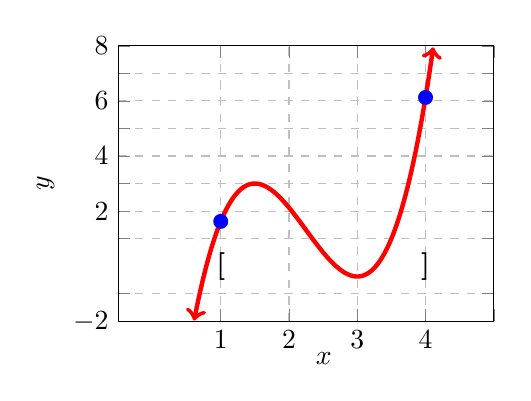
\begin{tikzpicture}[scale=1]
          \begin{axis}[
            xlabel={$x$},
            xlabel style={anchor=west},
            ylabel={$y$}, 
            ylabel style={anchor=south},
            %grid = major,
            xtick       = {1,2,3,4,5},
            xticklabels = {$1$,$2$,$3$,$4$},
            ytick       = {-2,-1,1,2,3,4,5,6,7,8},
            yticklabels = {$-2$,,,$2$,,$4$,,$6$,,$8$},
            samples     = 320,
            domain      = -.5:5,
            restrict y to domain=-2:8,
            xmin = -.5, xmax = 5,
            ymin = -2, ymax = 8,
            grid=both, grid style=dashed,
            height=2in, width=2.5in
          ]
          \addplot[domain=.51:4.5, ultra thick, red,<->] {  2*(x-1.5)^2*(x-3.75)+3  };
          \filldraw[blue] (1,1.625) circle (2.5pt);
          \filldraw[blue] (4,6.125) circle (2.5pt);
          \draw (1,0) node {  \blue{\textbf{[}} };
           \draw (4,0) node {  \blue{\textbf{]}} };
          %
        \end{axis}
    \end{tikzpicture}
    \end{flushleft}
    }{
\hs{.1}\# Local Mins \vs{.3}\\
\hs{.1}\# Local Maxs\vs{.3}\\
\hs{.1}\# Abs Mins \vs{.3}\\
\hs{.1}\# Abs Maxs
\blue{\\[.25em]
\# Local Mins: $1$ at $x=3$.\\
\# Local Maxs: $1$ at $x=\frac{3}{2}$.\\
\# Abs Mins: $1$ at $x=3$.\\
\# Abs Maxs: $1$ at $x=4$.}
}{
\begin{flushleft}
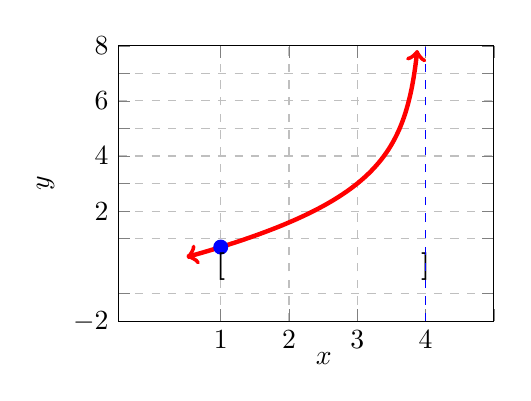
\begin{tikzpicture}[scale=1]
          \begin{axis}[
            xlabel={$x$},
            xlabel style={anchor=west},
            ylabel={$y$}, 
            ylabel style={anchor=south},
            %grid = major,
            xtick       = {1,2,3,4,5},
            xticklabels = {$1$,$2$,$3$,$4$},
            ytick       = {-2,-1,1,2,3,4,5,6,7,8},
            yticklabels = {$-2$,,,$2$,,$4$,,$6$,,$8$},
            samples     = 320,
            domain      = -.5:5,
            restrict y to domain=-2:8,
            xmin = -.5, xmax = 5,
            ymin = -2, ymax = 8,
            grid=both, grid style=dashed,
            height=2in, width=2.5in
          ]
          \addplot[domain=.5:4, ultra thick, red,<->] {  x/(4-x)^(1/3)  };
          \filldraw[blue] (1,.6933) circle (2.5pt);
%          \filldraw[blue] (4,6.125) circle (2.5pt);
          \draw (1,0) node {  \blue{\textbf{[}} };
           \draw (4,0) node {  \blue{\textbf{]}} };
           \draw[dashed, blue] (4,-2) -- (4,9);
          %
        \end{axis}
    \end{tikzpicture}
    \end{flushleft}
}{
\hs{.1}\# Local Mins \vs{.3}\\
\hs{.1}\# Local Maxs\vs{.3}\\
\hs{.1}\# Abs Mins \vs{.3}\\
\hs{.1}\# Abs Maxs
\blue{\\[.25em]
\# Local Mins: $0$.\\
\# Local Maxs: $0$.\\
\# Abs Mins: $1$ at $x=1$ (finite left endpoint value).\\
\# Abs Maxs: $0$ (as $x\to 4^{-}$, $f(x)\to +\infty$).}
}
~\\
\mpageTfour{.35}{.2}{.35}{.2}{
\begin{flushleft}
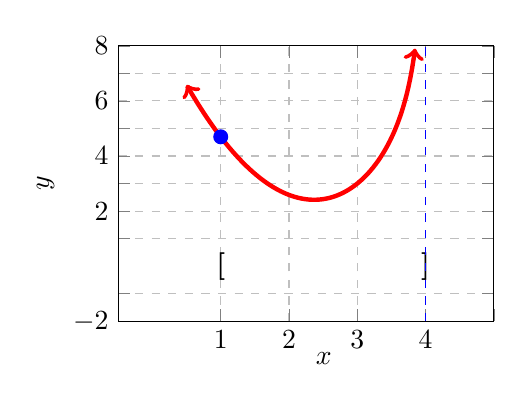
\begin{tikzpicture}[scale=1]
          \begin{axis}[
            xlabel={$x$},
            xlabel style={anchor=west},
            ylabel={$y$}, 
            ylabel style={anchor=south},
            %grid = major,
            xtick       = {1,2,3,4,5},
            xticklabels = {$1$,$2$,$3$,$4$},
            ytick       = {-2,-1,1,2,3,4,5,6,7,8},
            yticklabels = {$-2$,,,$2$,,$4$,,$6$,,$8$},
            samples     = 320,
            domain      = -.5:5,
            restrict y to domain=-2:8,
            xmin = -.5, xmax = 5,
            ymin = -2, ymax = 8,
            grid=both, grid style=dashed,
            height=2in, width=2.5in
          ]
          \addplot[domain=.5:4, ultra thick, red,<->] {  x/(4-x)^(1/3)+(x-3)^2 };
          \filldraw[blue] (1,4.696) circle (2.5pt);
%          \filldraw[blue] (4,6.125) circle (2.5pt);
          \draw (1,0) node {  \blue{\textbf{[}} };
           \draw (4,0) node {  \blue{\textbf{]}} };
             \draw[dashed, blue] (4,-2) -- (4,9);
          %
        \end{axis}
    \end{tikzpicture}
    \end{flushleft}
}{
\hs{.1}\# Local Mins \vs{.3}\\
\hs{.1}\# Local Maxs\vs{.3}\\
\hs{.1}\# Abs Mins \vs{.3}\\
\hs{.1}\# Abs Maxs
\blue{\\[.25em]
\# Local Mins: $1$ at $x\approx \frac{5}{2}$.\\
\# Local Maxs: $0$.\\
\# Abs Mins: $1$ at the same interior point $x\approx \frac{5}{2}$.\\
\# Abs Maxs: $0$ (function $\to +\infty$ as $x\to 4^{-}$).}
}{
\begin{flushleft}
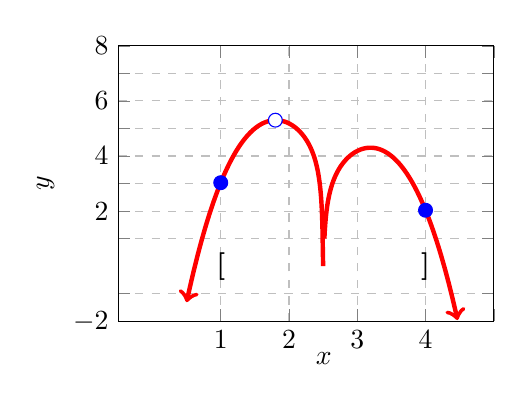
\begin{tikzpicture}[scale=1]
          \begin{axis}[
            xlabel={$x$},
            xlabel style={anchor=west},
            ylabel={$y$}, 
            ylabel style={anchor=south},
            %grid = major,
            xtick       = {1,2,3,4,5},
            xticklabels = {$1$,$2$,$3$,$4$},
            ytick       = {-2,-1,1,2,3,4,5,6,7,8},
            yticklabels = {$-2$,,,$2$,,$4$,,$6$,,$8$},
            samples     = 320,
            domain      = -.5:5,
            restrict y to domain=-2:8,
            xmin = -.5, xmax = 5,
            ymin = -2, ymax = 8,
            grid=both, grid style=dashed,
            height=2in, width=2.5in
          ]
          \addplot[domain=.5:2.49, ultra thick, red,<-] {  (x-5/2)^3+ln(5/2-x)+6  };
           \addplot[domain=2.5183:4.5, ultra thick, red,->] {  -(x-5/2)^3+ln(x-5/2)+5  };
           \draw[ultra thick, red] (2.49,1.39) -- (2.5,0);
          \filldraw[blue] (1,3.03) circle (2.5pt);
          \filldraw[blue] (4,2.03) circle (2.5pt);
                   \filldraw[blue, fill=white] (1.8,5.3) circle (2.5pt);
          \draw (1,0) node {  \blue{\textbf{[}} };
         \draw (4,0) node {  \blue{\textbf{]}} };
%           \draw[dashed, blue] (2.5,-2) -- (2.5,9);
          %
        \end{axis}
    \end{tikzpicture}
    \end{flushleft}
}{
\hs{.1}\# Local Mins \vs{.3}\\
\hs{.1}\# Local Maxs\vs{.3}\\
\hs{.1}\# Abs Mins \vs{.3}\\
\hs{.1}\# Abs Maxs
\blue{\\[.25em]
\# Local Mins: $1$ at $x \approx \frac{5}{2}$. (The derivative DNE there)\\
\# Local Maxs: $1$ at $x \approx \frac{10}{3}$. (The function is not defined at the other potential local max at $x \approx \frac{5}{3}$).\\
\# Abs Mins: $1$ at $x \approx \frac{5}{2}$ ($\displaystyle \lim_{x \to \frac{5}{2}}f(x) = 0$).\\
\# Abs Maxs: $0$ (No point $c \in [1,4]$ satisfies the definition).}
}
~\\
 ({\bf Extreme Value Theorem}) {\bf If} $f$ is {\em continuous} on $[a,b]$, {\bf then} $f$ attains an absolute maximum and minimum somewhere on $[a,b]$
\vs{.3}\\
{\em Key Observations}\vs{.5}\\
%{\em Practical Tips}
\blue{
\begin{itemize}
    \item \textcolor{blue}{A function may have \emph{local extrema} (local maxima or minima) inside an interval, even if they are not absolute extrema.}
    \item \textcolor{blue}{Absolute extrema (global max/min) must occur either at \emph{critical points} (where $f'(x)=0$ or $f'(x)$ does not exist) or at the \emph{endpoints} of the interval.}
    \item \textcolor{blue}{The Extreme Value Theorem (EVT) guarantees the existence of both an absolute maximum and minimum \textbf{only if $f$ is continuous on a closed interval $[a,b]$}.}
    \item \textcolor{blue}{If $f$ is not continuous on $[a,b]$, then absolute extrema might fail to exist, even if local extrema do.}
    \item \textcolor{blue}{Discontinuities, vertical asymptotes, or open endpoints can prevent the function from attaining its absolute maximum or minimum.}
    \item \textcolor{blue}{Local extrema depend on the \textit{shape} of the graph (turning points), whereas absolute extrema depend on the \textit{overall range} of function values on the interval.}
    \item \textcolor{blue}{At an endpoint, a one-sided comparison is used to determine if the endpoint is a local or absolute extremum.}
    \item \textcolor{blue}{Functions that grow without bound on $[a,b]$ (e.g., $f(x)\to +\infty$ near $b$) do \textbf{not} have an absolute maximum, even though they may have a finite absolute minimum.}
\end{itemize}
}

\newpage

{\bf \blue{ Practical Tips:} Closed Interval Method.} To find the absolute maximum value and absolute minimum value of a continuous function $f$ on the closed interval $[a, b]$, do the following:
\smallskip

\begin{minipage}{0.75\textwidth}
\enum{
\item  Find the critical numbers $c_1, c_2, \ldots, c_n$ of $f$ that lie in $(a, b)$.
\item  Find the value of $f$ at each critical number {\em and} at the endpoints


\item  The largest value from $2$)  will be the absolute maximum value of $f$ on $[a, b]$ and the smallest vakye will be the absolute minimum value of $f$ on $[a, b]$. 
}
\end{minipage}
%
\hfill
%
\begin{minipage}{0.2\textwidth}
\begin{center}
\begin{tabular}{|c|c|}
\hline 
$x$ & $f(x)$\tabularnewline
\hline 
\hline 
$a$ & $f(a)$\tabularnewline
\hline 
$b$ & $f(b)$\tabularnewline
\hline 
$c_1$ & $f(c_1)$\tabularnewline
\hline 
$c_2$ & $f(c_2)$\tabularnewline
\hline 
$\vdots$ &$\vdots $\tabularnewline
\hline 
$c_n$ & $f(c_n)$\tabularnewline
\hline 
\end{tabular}
\end{center}
\end{minipage}
\bigskip

 {\example}\ltrm{\color{RedOrange}A2} Find the absolute maximum and absolute minimum values of $f(x)=\sqrt[3]{x^2-4x}$, where $x$ is in $[-1,3]$.
\blue{\\[.5em]\textbf{Solution:} We proceed using the\textbf{ Closed Interval Method}.
Let $u(x)=x^2-4x$. Then $f(x)=u(x)^{1/3}$, so
\[
f'(x)=\tfrac{1}{3}u(x)^{-2/3}\cdot u'(x)=\tfrac{1}{3}(x^2-4x)^{-2/3}(2x-4).
\]
Critical points in $(-1,3)$ occur when $2x-4=0 \iff x=2$ and where $f'$ is undefined but $f$ is defined, i.e., $x^2-4x=0\Rightarrow x=0$ (note $x=4\notin [-1,3]$). Now, we need to check the endpoints $x = -1$ and $x = 3$ Evaluate:
\[
\begin{aligned}
f(-1)&=\sqrt[3]{5} ,\\
f(0)&=0,\\
f(2)&=\sqrt[3]{-4}=-\sqrt[3]{4},\\
f(3)&=\sqrt[3]{-3}=-\sqrt[3]{3}.
\end{aligned}
\]
Compare: $-\sqrt[3]{4}<-\sqrt[3]{3}<0<\sqrt[3]{5}$.\\
\textbf{Absolute min:} $f(2)=-\sqrt[3]{4}$ at $x=2$. \quad
\textbf{Absolute max:} $f(-1)=\sqrt[3]{5}$ at $x=-1$.}

\vfill
 
 

{\exercise}\ltrm{\color{RedOrange}A2} Find the absolute maximum and absolute minimum values of $\ds f(x)=\frac{1}{3}x^3-2x^2+\frac{5}{3}$ on the interval $[-1,1]$.   
\blue{\\[.5em]\textbf{Solution:} We again proceed using the\textbf{ Closed Interval Method}. The derivative, $f'(x)=x^2-4x=x(x-4)$. There's no $x$-values where $f'(x)$ DNE. So, the only critical number in $(-1,1)$ is  $x=0$. Next, evaluate at the critical numbers along with the endpoints:
\[
f(-1)=-\tfrac{1}{3}-2+\tfrac{5}{3}=-\tfrac{2}{3},\quad
f(0)=\tfrac{5}{3},\quad
f(1)=\tfrac{1}{3}-2+\tfrac{5}{3}=0.
\]
\textbf{Absolute max:} $f(0)=\tfrac{5}{3}$ at $x=0$. \quad
\textbf{Absolute min:} $f(-1)=-\tfrac{2}{3}$ at $x=-1$.}
    \vfill
    
{\exercise}\ltrm{\color{RedOrange}A2} Find the absolute maximum and absolute minimum values of $\ds g(x)=x^2+\frac{128}{x}$ on the interval $[1,8]$.
\blue{\\[.5em]\textbf{Solution:} The derivative is given by $g'(x)=2x-\dfrac{128}{x^2}$. Set $g'(x)=0$:
\[
2x=\frac{128}{x^2}\ \Longrightarrow\ 2x^3=128\ \Longrightarrow\ x^3=64\ \Longrightarrow\ x=4.
\]
Since the only point where $g'(x)$ DNE is when $x = 0$ and it is not in the domain of definition, we may disregard this potential critical point.
Next, we evaluate at the critical points along with the endpoints of the given interval: $g(1)=129$, $g(4)=16+32=48$, $g(8)=64+16=80$.\\
\textbf{Absolute min:} $g(4)=48$ at $x=4$. \quad
\textbf{Absolute max:} $g(1)=129$ at $x=1$.}
    
    \vfill
    
\newpage

{\bf\color{blue} Non-closed intervals.} The Extreme Value Theorem applies only to functions that are continuous on closed intervals. So it's possible the function at hand might not have  an absolute maximum/minimum. In such cases we may use limits to determine the behavior of the function at its excluded endpoint(s).\\

\blue{\bf Example/}\hs{-.15}{\exercise}\ltrm{\color{RedOrange}A2} Consider the following to explore what happens when our interval is not closed.\\
\mpageT{.6}{.4}{
\begin{itemize}
\item[i.] How do the answers to Exercise A change if instead the interval is $(-1,1]$?   $(-1,0))$?\\[0.05in]
%
\fbox{
\begin{minipage}{0.375\textwidth}
\begin{center}$\mathbf{(-1,1]}$\end{center}\vs{-.15}
Abs. max:\unline{.75}{}{.25}\\[0.25in]
Abs. min:\unline{.75}{}{.25}\\[0.25in]
\end{minipage}
}
%\hfill
\fbox{
\begin{minipage}{0.375\textwidth}
\begin{center}$\mathbf{(-1,0)}$\end{center}\vs{-.15}
Abs. max:\unline{.75}{}{.25}\\[0.25in]
Abs. min:\unline{.75}{}{.25}\\[0.25in]
\end{minipage}
}
\vs{.2}
\item[ii.] How do the answers to Exercise B change if instead the interval is $[1,\infty]$?   $(6,10]$?\\[0.05in]
%
\fbox{
\begin{minipage}{0.375\textwidth}
\begin{center}$\mathbf{[1,\infty)}$\end{center}\vs{-.15}
Abs. max:\unline{.75}{}{.25}\\[0.25in]
Abs. min:\unline{.75}{}{.25}\\[0.25in]
\end{minipage}
}
%\hfill
\fbox{
\begin{minipage}{0.375\textwidth}
\begin{center}$\mathbf{(6,10]}$\end{center}\vs{-.15}
Abs. max:\unline{.75}{}{.25}\\[0.25in]
Abs. min:\unline{.75}{}{.25}\\[0.25in]
\end{minipage}
}
\end{itemize}
}{
\begin{flushright}
\begin{tikzpicture}[scale=1]
          \begin{axis}[
            xlabel={$x$},
            xlabel style={anchor=west},
            ylabel={$f(x)=\dfrac{1}{3}x^3-2x^2+\frac{5}{3}$}, 
            ylabel style={anchor=south},
            %grid = major,
            xtick       = {-2,-1,1,2},
            xticklabels = {$-2$,,$1$,$2$},
            ytick       = {-4,-2,2,4},
            yticklabels = {$-4$,$-2$,,$4$},
            samples     = 320,
            domain      = -2:2,
            restrict y to domain=-4:4,
            xmin = -2.5, xmax = 2.5,
            ymin = -4, ymax = 4,
            grid=both, grid style=dashed,
            height=2in, width=2.5in
          ]
          \addplot[domain=-2:2, ultra thick, red,<-] {  1/3*x^3-2*x^2+5/3  };
                    \filldraw[blue] (0,5/3) circle (2.5pt);
          \filldraw[blue] (-1,-2/3) circle (2.5pt);
       \draw (.2,2.2) node[anchor=west] {\small $f(0)=\dfrac{5}{3}$ };
           \draw (-.5,1.6) node[anchor=east] {\small $f(-1)=-\dfrac{2}{3}$ };
               \draw[blue,-latex] (-1.5,1) -- (-1.1,-.4);
%          \draw (-1,0) node {\Large  \blue{\textbf{[}} };
%           \draw (1,0) node { \Large \blue{\textbf{]}} };
          %
        \end{axis}
    \end{tikzpicture}
    \end{flushright}
  %  ~\\
  \vs{.2}
    \begin{flushright}
\begin{tikzpicture}[scale=1]
          \begin{axis}[
            xlabel={$x$},
            xlabel style={anchor=west},
           y axis line style={thick, blue, dashed},
            ylabel={$\qquad g(x)=x^2+\dfrac{128}{x}$}, 
            ylabel style={anchor=south west},
            %grid = major,
            xtick       = {2,4,6,8,10},
            xticklabels = {$2$,$4$,$6$,$8$,$10$},
            ytick       = {50,100,150,200,250,300},
            %yticklabels = {$50$,$-2$,,$4$},
            samples     = 320,
%            domain      = 0:10,
            restrict y to domain=0:300,
            xmin = 0, xmax = 11,
            ymin = -20, ymax = 300,
            grid=both, grid style=dashed,
            height=2in, width=2.5in
          ]
          \addplot[domain=.4:11, ultra thick, red,<->] {  x^2+128/x  };
                    \filldraw[blue] (4,48) circle (2.5pt);
          \filldraw[blue] (6,57.33) circle (2.5pt);
           \filldraw[blue] (10,112.8) circle (2.5pt);
       \draw (5,125) node[anchor=east] {\small $g(4)=48$ };
              \draw[blue,-latex] (3.5,110) -- (4,58);
               \draw (6,150) node[anchor=south] {\small $g(6)=57\dfrac{1}{3}$};
               \draw[blue,-latex] (6,175) -- (6,70);
                 \draw (11,250) node[anchor=east] {\small $g(10)=112.8$};
                   \draw[blue,-latex] (8.75,235) -- (9.9,125);
%          \draw (-1,0) node {\Large  \blue{\textbf{[}} };
%           \draw (1,0) node { \Large \blue{\textbf{]}} };
          %
        \end{axis}
    \end{tikzpicture}
    \end{flushright}
}
\vs{.2}~\\
\blue{\bf Solutions:}
\blue{
\begin{itemize}
\item[(i)] On $(-1,1]$: \textbf{Abs.\ max} $f(0) = \dfrac{5}{3}$ (included); \textbf{Abs.\ min} does \emph{not} exist ($\displaystyle \lim_{x \to -1^{+}}f(x) = -2/3$ at is not attained and there are values in the interval which are smaller than $f(1)$).\\
On $(-1,0)$: \textbf{Abs.\ max} does not exist ($\displaystyle \lim_{x \to 0^{-}} f(x)=5/3$ is not attained); \textbf{Abs.\ min} does not exist ($\displaystyle \lim_{x \to -1^{+}} f(x)=-2/3$ is not attained. There are no candidates for a largest or smallest value on the (open) interval in question).
\item[(ii)] On $[1,\infty)$: \textbf{Abs.\ min} $g(4)=48$; \textbf{Abs.\ max} does not exist ($g(x)\to\infty$ as $x\to\infty$ and also as $x \to 1$).\\
On $(6,10]$: $g'(x)>0$ so $g$ increases; \textbf{Abs.\ max} $=g(10)=112.8$; \textbf{Abs.\ min} does not exist ($\displaystyle \lim_{x \to 6^{+}}f(x) = 57 \frac{1}{3}$ is excluded).
\end{itemize}
}

\blue{\bf Reflect} Based on the above Discussion, how would you describe the process of finding absolute extrema on non-closed intervals? 
\blue{
\textbf{Process for Finding Absolute Extrema on Non-Closed Intervals:}\\[0.5em]
When the interval is not closed, the Extreme Value Theorem does not guarantee the existence of absolute maxima or minima. 
To analyze such cases:
\begin{itemize}
    \item Identify and evaluate all \emph{critical points} of $f$ that lie within the open or half-open interval.
    \item Examine the \emph{behavior near excluded endpoints} using limits. 
    For example, if $a$ is excluded, consider $\displaystyle \lim_{x \to a^{+}} f(x)$ (or $\lim_{x \to a^{-}} f(x)$) to see whether the function approaches a finite value or diverges.
    \item If the limit exists and is finite, it can describe the \emph{trend} of $f$ near the endpoint, but it does not count as an attained absolute extremum since the endpoint is not included.
    \item Compare the function values at all included endpoints (if any) and at interior critical points to determine which are the largest or smallest \emph{attained} values.
    \item If $f(x)$ grows without bound or approaches but never reaches a limiting value, then the corresponding absolute maximum or minimum \textbf{does not exist}.
\end{itemize}
In summary, for non-closed intervals, we use limits to describe boundary behavior, but only \emph{attained} values at interior points or included endpoints can be considered absolute extrema.
}

%%%%%%%%%
%%%%%%%%%

 \mpageT{.5}{.5}{
\important{First Derivative Test for Absolute Extrema}
{
Suppose that $c$ is a critical number of a continuous function $f$ defined on an interval $I$.
    \begin{itemize}
    \item {\bf If} the sign of $f'$ changes from positive ($+$) to negative ($-$) at $c$ {\bf and} $c$ is the only critical number where $f^{\prime}$ changes sign on $I$
    %\emph{and} if $c$ is the only $x$-value in $I$ at which $f$ changes sign, 
    {\bf then} $f(c)$ is the absolute maximum value of $f$ on $I$.
    \item {\bf If} the sign of $f'$ changes from negative ($-$) to positive ($+$) at $c$ {\bf and} $c$ is the only critical number where $f^{\prime}$ changes sign on $I$
    % \emph{and} if $c$ is the only $x$-value in $I$ at which $f$ changes sign, 
    {\bf then} $f(c)$ is the absolute minimum value of $f$ on $I$.\\
    \end{itemize}
}
}{
}

\vs{.2}~\\
{\exercise}\ltrm{\color{RedOrange}A2} In {\bf Exercise A} we examined the function $f(x)=\dfrac13x^3-2x^2+\dfrac53$ and found $$f^{\prime}(x)=x^2-4x=x(x-4)$$ with critical numbers at $x=0,4$. We're going to utilize the First Derivative Test for Absolute Extrema to determine if $f$ has absolute max/mins on the interval $(0,9)$.
\enum{
\mpageT{.7}{.3}[\hs{.1}]{
\item Create a sign line for $f^{\prime}$ for the given interval and critical number(s) in that interval.
}{\begin{flushright}
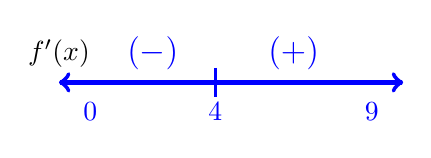
\begin{tikzpicture}
    \begin{axis}[
    	axis x line=none,
	            axis y line=none,
		x label style={anchor=west},
            xlabel={},
            xtick       = {0},
            xticklabels = {$c$},
            y label style={anchor=south},
            ylabel={},
            ytick       = {-6,-4,-2,2,4,6},
            yticklabels = {$-6$,$-4$,$-2$,$2$,$4$,$6$},
            samples     = 320,
            domain      = -1:10,
            restrict y to domain=-6.5:6.5,
            xmin = -2, xmax = 10,
            ymin = -6.5, ymax = 6.5,
            width=2.5in, height=2.5in,
            grid=none, grid style=solid
          ]
    \addplot[domain=-1:10, blue, ultra thick, mark=none, <->]{0)};
	\draw (-1,1) node{$\Large f^{\prime}(x)$};
	\draw[blue, very thick] (4,0.5) -- (4,-0.5);
	\node[below, blue] at (4,-0.35) {$4$};
	\node[below, blue] at (0,-0.35) {$0$};
	\node[below, blue] at (9,-0.35) {$9$};
	\node[blue] at (2,1) {\large $(-)$};
	\node[blue] at (6.5,1) {\large $(+)$};
    \end{axis}
\end{tikzpicture}
\end{flushright}
}
\blue{~\\[.5em]\textbf{Solution}
For $(0,9)$ the only sign change occurs at $x=4$ (since $x=0$ is not in the interval). Test signs: choose $x=1$ gives $f'(1)=1-4<0$; choose $x=5$ gives $f'(5)=25-20>0$. Thus $f'$ changes from $-$ to $+$ at $x=4$.}
\item What, if anything, can we conclude from the First Derivative Test for Absolute Extrema? Do we have both an Absolute Max and an Absolute Min?

\blue{\textbf{Solution}
\begin{itemize}
%\item For $(0,9)$ the only sign change occurs at $x=4$ (since $x=0$ is not in the interval). Test signs: choose $x=1$ gives $f'(1)=1-4<0$; choose $x=5$ gives %$f'(5)=25-20>0$. Thus $f'$ changes from $-$ to $+$ at $x=4$.
\item By the First Derivative Test for Absolute Extrema (and uniqueness of the sign change in $(0,9)$), $f(4)$ is the \textbf{absolute minimum} on $(0,9)$.
\item Compute $\ds f(4)=\frac{1}{3}\cdot 64-2\cdot 16+\frac{5}{3}=\frac{64+5}{3}-32=\frac{69}{3}-32=23-32=-9$.
\item There is \textbf{no absolute maximum} on $(0,9)$: $f$ decreases on $(0,4]$ and increases on $[4,9)$. Since $x=0$ is excluded, the local max at $0$ from $[-1,1]$ is not available.
\end{itemize}
}
}
\newpage

{\bf\color{blue}Extra Practice 1.}\ltrm{\color{RedOrange}A2} Find the absolute extrema of $M(x)=2x-6\sqrt{x}$ on the interval $[0,\infty)$.
\blue{\\[.5em]\textbf{Solution} $M'(x)=2-\dfrac{6}{2\sqrt{x}}=2-\dfrac{3}{\sqrt{x}}$. Set $M'(x)=0\Rightarrow \sqrt{x}=\tfrac{3}{2}\Rightarrow x=\tfrac{9}{4}$. Evaluate:
\[
M(0)=0,\quad M\!\left(\tfrac{9}{4}\right)=2\cdot\tfrac{9}{4}-6\cdot\tfrac{3}{2}= \tfrac{9}{2}-9=-\tfrac{9}{2}.
\]

$M'(x)$ DNE at $x = 0$, but since this is an endpoint, we can test it using $M(x)$. 
Checking the sign line below, we've:
$M'(1) = -1$ and $M'(9) = 1$
As $x\to\infty$, $M(x)\sim 2x\to\infty$. Hence \textbf{absolute min:} $M(\frac{9}{4})=-\dfrac{9}{2}$; \textbf{no absolute max} (unbounded above).}
\vfill

%Based on our conclusions above, let's modify the Closed Interval Method to include certain cases when the interval is {\it not} closed.\\

%{\bf Modified Closed Interval Method.} To find the absolute maximum value and absolute minimum value of a continuous function $f$ on the closed interval $[a, b]$, do the following:
%\smallskip
%
%\begin{minipage}{0.75\textwidth}
%\begin{itemize}
%\item[(i)]  Find the critical numbers $c_1, c_2, \ldots, $c_n$ of $f$ that lie in $(a, b)$.
%\item[(ii)]  Make an {\it outputs table} consisting of the values of $f$ at the  endpoints $a$ and $b$ as well as at each critical number inside $(a, b)$ (identified in (i)).
%
%\smallskip
%
%\item[(iii)]  The largest output (in the right column) in the outputs table of (ii) will be the absolute maximum value of $f$ on $[a, b]$ and the smallest output in the outputs table will be the absolute minimum value of $f$ on $[a, b]$. 
%\end{itemize}
%\end{minipage}
%%
%\hfill
%%
%\begin{minipage}{0.2\textwidth}
%\begin{center}
%\begin{tabular}{|c|c|}
%\hline 
%$x$ & $f(x)$\tabularnewline
%\hline 
%\hline 
%$a$ & $f(a)$\tabularnewline
%\hline 
%$b$ & $f(b)$\tabularnewline
%\hline 
%$c_1$ & $f(c_1)$\tabularnewline
%\hline 
%$c_2$ & $f(c_2)$\tabularnewline
%\hline 
%$\vdots$ &$\vdots $\tabularnewline
%\hline 
%$c_n$ & $f(c_n)$\tabularnewline
%\hline 
%\end{tabular}
%\end{center}
%\end{minipage}
%
%\begin{itemize}
%
%\item[(iv)] If all $x$-values at which an absolute extremum occurs are removed from the interval, then that absolute extremum \rule[-8pt]{0.5in}{0.4pt} on the modified interval. Otherwise, that absolute extremum is preserved on the modified interval.
%
%\end{itemize}


\begin{tikzpicture}[scale=1.2]
    % Draw the horizontal sign line
    %\draw[thick, blue, -latex] (0,0) -- (6.1,0);
    \draw[blue, thick] (0,0) -- (9,0);
    
    % Critical points (x = 0, 4)
    %\foreach \x in {0,4}{
     %   \draw[blue, thick] (\x,0.25) -- (\x,-0.25);
    %}
    \draw[blue, very thick] (2.25,0.25) -- (2.25,-0.25);

    % Labels for x-values
    \node[below, blue] at (0,-0.25) {$0$};
    \node[below, blue] at (2.25,-0.45) {$\frac{9}{4}$};
    \node[below, blue] at (6,-0.25) {$9$};
    
    % Interval signs
    \node[blue] at (1.3,0.5) {\Large $-$};
    \node[blue] at (5,0.5) {\Large $+$};
    
    % Function label
    \node[above left, blue] at (-0.5,0.5) {$f'(x)$};
    
    % Arrows for direction of intervals
   % \draw[blue, thick, -latex] (0.2,0.6) -- (1.5,0.6);
   % \draw[blue, thick, -latex] (4.2,0.6) -- (5.5,0.6);
\end{tikzpicture}

{\bf\color{blue}Extra Practice 2.}\ltrm{\color{RedOrange}A2} Find the absolute extrema of $f(x)=x+\dfrac{16}{x}$ on the interval $(0,\infty)$.
\blue{\\[.5em]\textbf{Solution} $f'(x)=1-\dfrac{16}{x^2}$. Set $f'(x)=0\Rightarrow x^2=16\Rightarrow x=4$ (only positive root). Evaluate:
\[
f(4)=4+4=8,\qquad f(x)\to\infty\ \text{as }x\to 0^+\ \text{or }x\to\infty.
\]
Note that $f'$ DNE at $x = 0$ but that point is not in the domain of $f$. Using a sign line, we've $f'(1) = -15$ and $f'(5) = \frac{9}{25}$

\begin{tikzpicture}[scale=1.2]
    % Draw the horizontal sign line
    %\draw[thick, blue, -latex] (0,0) -- (6.1,0);
    \draw[blue, thick] (0,0) -- (9,0);
    
    % Critical points (x = 0, 4)
    %\foreach \x in {0,4}{
     %   \draw[blue, thick] (\x,0.25) -- (\x,-0.25);
    %}
    \draw[blue, very thick] (2.25,0.25) -- (2.25,-0.25);

    % Labels for x-values
    \node[below, blue] at (0,-0.25) {$0$};
    \node[below, blue] at (2.25,-0.45) {$4$};
    \node[below, blue] at (6,-0.25) {$9$};
    
    % Interval signs
    \node[blue] at (1.8,0.5) {\Large $-$};
    \node[blue] at (5,0.5) {\Large $+$};
    
    % Function label
    \node[above left, blue] at (-0.5,0.5) {$f'(x)$};
    
    % Arrows for direction of intervals
   % \draw[blue, thick, -latex] (0.2,0.6) -- (1.5,0.6);
   % \draw[blue, thick, -latex] (4.2,0.6) -- (5.5,0.6);
\end{tikzpicture}

Thus \textbf{absolute minimum:} $f(4)=8$; \textbf{no absolute maximum}.
}

\vfill

{\bf\color{blue}Extra Practice 3.}\ltrm{\color{RedOrange}A2} Find the absolute extrema of $f(x)=\dfrac{1}{x^2-2x+2}$ on the intervals below:\\[0.1in]
%
\,\hfill
%
\fbox{
\begin{minipage}{0.15\textwidth}
\begin{center}
{\Large$\left[-1,2\right]$}
\end{center}
max: \rule[-8pt]{0.5in}{0.4pt}\\[0.2in]
min: \,\rule[-8pt]{0.5in}{0.4pt}
\end{minipage}
}
%
\hfill
%
\fbox{
\begin{minipage}{0.15\textwidth}
\begin{center}
{\Large$\left[-1,2\right)$}
\end{center}
max: \rule[-8pt]{0.5in}{0.4pt}\\[0.2in]
min: \,\rule[-8pt]{0.5in}{0.4pt}
\end{minipage}
}
%
\hfill
%
\fbox{
\begin{minipage}{0.15\textwidth}
\begin{center}
{\Large$\left(-1,2\right]$}
\end{center}
max: \rule[-8pt]{0.5in}{0.4pt}\\[0.2in]
min: \,\rule[-8pt]{0.5in}{0.4pt}
\end{minipage}
}
%
\hfill
%
\fbox{
\begin{minipage}{0.15\textwidth}
\begin{center}
{\Large$\left(-1,2\right)$}
\end{center}
max: \rule[-8pt]{0.5in}{0.4pt}\\[0.2in]
min: \,\rule[-8pt]{0.5in}{0.4pt}
\end{minipage}
}
%
\hfill\,\\[0.2in]
%

\vfill

\bigskip

\blue{
\textbf{Solutions}

\medskip

We work with
\[
f(x)=\frac{1}{x^2-2x+2}=\frac{1}{(x-1)^2+1}.
\]
Note first that the denominator $(x-1)^2+1>0$ for all real $x$, so $f$ is continuous everywhere and well defined on all the given intervals.

\medskip

\textbf{1. Find critical numbers.}

Differentiate using the chain/quotient rule (or differentiate the form $( (x-1)^2+1)^{-1}$):
\[
f(x)=\big((x-1)^2+1\big)^{-1}\quad\Longrightarrow\quad
f'(x)=-1\cdot\big((x-1)^2+1\big)^{-2}\cdot 2(x-1).
\]
Thus
\[
\boxed{\,f'(x)=\displaystyle -\frac{2(x-1)}{\big((x-1)^2+1\big)^2}\, }.
\]

Set \(f'(x)=0\). The denominator is never zero, so numerator must be zero:
\[
-2(x-1)=0 \quad\Longrightarrow\quad x=1.
\]
So the only critical number is \(x=1\).

\medskip
\bigskip


\textbf{2. Determine sign of \(f'(x)\) using a sign line.}\\[4pt]
Since the denominator $\big((x-1)^2+1\big)^2>0$ for all $x$, the sign of $f'(x)$ depends only on the numerator $-2(x-1)$.
Thus: 
\[
\begin{cases}
f'(x)>0, & \text{if }x<1,\\[4pt]
f'(x)=0, & \text{if }x=1,\\[4pt]
f'(x)<0, & \text{if }x>1.
\end{cases}
\]

\medskip
We represent this with the following sign line:


\begin{center}
\begin{tikzpicture}[scale=1.2]
  % Draw the base number line
  \draw[blue, thick, -] (-3,0) -- (3,0);

  % Mark the critical point x=1 (centered at 0 on the drawn axis for convenience)
  \draw[blue, thick] (0,-0.15) -- (0,0.15);
  \node[below, blue] at (0,-0.2) {$x=1$};

  % Add plus and minus regions
  \node[blue] at (-1.8,0.4) {\Large $+$};
  \node[blue] at (1.8,0.4) {\Large $-$};

  % Add directional arrows to indicate monotonicity
  %\draw[blue, thick, -latex] (-2.8,0.4) -- (-2,0.4);
  %\draw[blue, thick, -latex] (1,0.4) -- (2.8,0.4);

  % Label the derivative
  \node[above, blue] at (0,1) {\large $f'(x) = -\dfrac{2(x-1)}{((x-1)^2+1)^2}$};
\end{tikzpicture}
\end{center}
}
\blue{
\noindent
From the sign line, $f'$ changes from $+$ to $-$ at $x=1$, ($f'(0) = \frac{1}{2}$ and $f'(2) = -\frac{1}{2}$) so $f$ is increasing on $(-\infty,1)$ and decreasing on $(1,\infty)$, confirming that $x=1$ is a local (and in fact global) maximum.





Now evaluate $f(1)=1$ and proceed to the endpoints for each interval.


\textbf{3. Evaluate \(f\) at the relevant endpoints.}

Compute values at the endpoints that occur in the four intervals:

\[
\begin{aligned}
f(-1)&=\frac{1}{(-1-1)^2+1}=\frac{1}{(-2)^2+1}=\frac{1}{4+1}=\frac{1}{5},\\[6pt]
f(2)&=\frac{1}{(2-1)^2+1}=\frac{1}{1^2+1}=\frac{1}{2}.
\end{aligned}
\]

Note the ordering of these values:
\[
\frac{1}{5}=0.2 < \frac{1}{2}=0.5 < 1.
\]

%Since \(f\) decreases as \(|x-1|\) increases, the smallest value on any closed interval containing \(-1\) will be at \(-1\) (because \(-1\) is farther from 1 %than 2 is).

\medskip

\textbf{4. Conclusions on each interval}

\begin{itemize}
  \item \(\mathbf{[-1,2]}\): This is a closed interval and \(f\) is continuous, so EVT applies. Candidates for absolute extrema are interior critical points and endpoints.
    \begin{itemize}
      \item \(f(1)=1\) (interior critical point) — largest of the three values.
      \item \(f(-1)=\tfrac{1}{5}\), \; \(f(2)=\tfrac{1}{2}\).
    \end{itemize}
    Therefore
    \[
    \boxed{\text{max } = 1 \text{ at } x=1,\qquad \text{min } = \frac{1}{5} \text{ at } x=-1.}
    \]

  \item \(\mathbf{[-1,2)}\): Left endpoint \(-1\) is included, right endpoint \(2\) is excluded.
    \begin{itemize}
      \item \(x=1\) (interior) gives \(f(1)=1\) so the absolute maximum still exists: \(\max=1\) at \(x=1\).
      \item The smallest value among attained values on this half-open interval is still \(f(-1)=\tfrac{1}{5}\) (since \(-1\) is included). Values arbitrarily close to \(2\) from the left give values near \(f(2)=\tfrac{1}{2}\), but \(f(2)\) itself is not in the interval — that does not affect the minimum because \(\tfrac{1}{5}<\tfrac{1}{2}\).
    \end{itemize}
    Therefore
    \[
    \boxed{\text{max } = 1 \text{ at } x=1,\qquad \text{min } = \frac{1}{5} \text{ at } x=-1.}
    \]

  \item \(\mathbf{(-1,2]}\): Left endpoint \(-1\) is excluded, right endpoint \(2\) is included.
    \begin{itemize}
      \item \(x=1\) is interior, so \(\max=1\) at \(x=1\) (attained).
      \item The value \(\tfrac{1}{5}\) is not attained on this interval because values \(f(x)\) for \(x\) approaching \(-1^+\) approach \(\tfrac{1}{5}\), but \(-1\) is not in the interval so $\displaystyle\lim_{x\to -1^{+}}f(x) = \frac{1}{5}$ is \emph{not attained}. The right endpoint gives \(f(2)=\tfrac{1}{2}\), which is larger than \(\tfrac{1}{5}\).
    \end{itemize}
    Therefore
    \[
    \boxed{\text{max } = 1 \text{ at } x=1,\qquad \text{min does not exist.}}
    \]

  \item \(\mathbf{(-1,2)}\): Both endpoints are excluded but \(x=1\) lies in the interval.
    \begin{itemize}
      \item \(x=1\) gives \(f(1)=1\) so the absolute maximum exists (and is attained) on this open interval.
      \item The smallest possible value would be the $\displaystyle\lim_{x\to -1^{+}}f(x) = \frac{1}{5}$, but since \(-1\) is not included, there is no attained minimum. (Similarly, approaching \(2^-\) yields values near \(\tfrac{1}{2}\), still larger than \(\tfrac{1}{5}\).)
    \end{itemize}
    Therefore
    \[
    \boxed{\text{max } = 1 \text{ at } x=1,\qquad \text{min does not exist}}
    \]
\end{itemize}

\medskip

\textbf{Final summary of answers:}
\[
\begin{aligned}
&[-1,2]: &&\text{max}=1\ \text{at }x=1,\quad \text{min}=\tfrac{1}{5}\ \text{at }x=-1.\\
&[-1,2): &&\text{max}=1\ \text{at }x=1,\quad \text{min}=\tfrac{1}{5}\ \text{at }x=-1.\\
&(-1,2]: &&\text{max}=1\ \text{at }x=1,\quad \text{min does not exist}.\\
&(-1,2): &&\text{max}=1\ \text{at }x=1,\quad \text{min does not exist}.
\end{aligned}
\]
}

% end \textcolor{blue}


%%%%%%%%%
\newpage%
%%%%%%%%%

{\bf\color{blue}Extra Practice 4.}\ltrm{\color{RedOrange}A2} Let $f(x)=24\ln(x)+x^3$. Find the absolute extrema of $f(x)$ over $(0,3]$. ({\bf Hint:} do you recall what happens to the graph of the natural logarithmic function as its input approaches $0$ from the right?)
%\bigskip
%
%\textcolor{blue}{%
%\section*{Extra Practice 4 --- Solution (all work shown)}%
%}
\medskip \\
\blue{
\textbf{Solution}
Let
\[
f(x)=24\ln(x)+x^3,\qquad x\in(0,3].
\]

\medskip

\textbf{1. Compute the derivative.}
\[
f'(x)=\frac{24}{x}+3x^2.
\]

\medskip

\textbf{2. Determine critical points and sign of \(f'\).}

Solve \(f'(x)=0\) for \(x>0\):
\[
\frac{24}{x}+3x^2=0 \quad\Longrightarrow\quad \frac{24}{x}=-3x^2.
\]
The left-hand side \(\frac{24}{x}>0\) for \(x>0\) while the right-hand side \(-3x^2\le 0\). Thus there is \emph{no solution} for \(x>0\). Therefore there are no critical numbers in \((0,3]\) coming from \(f'(x)=0\) and although $f'(0)$ DNE, it is not in the domain of $f$.

Moreover, for every \(x>0\) we have
\[
f'(x)=\frac{24}{x}+3x^2>0,
\]
so \(f'(x)\) is strictly positive on the entire interval \((0,3]\). Hence \(f\) is strictly increasing on \((0,3]\).
\medskip

\textbf{3. Endpoint / limit behavior.}

As \(x\to 0^{+}\), \(\ln(x)\to -\infty\), hence
\[
\lim_{x\to 0^{+}} f(x)=\lim_{x\to 0^{+}} \big(24\ln x + x^3\big) = -\infty.
\]
This shows \(f\) is unbounded below on \((0,3]\), so there is no absolute minimum.

The interval includes the right endpoint \(x=3\). Since \(f\) is strictly increasing on \((0,3]\), the largest value on the interval is attained at the right endpoint \(x=3\). Evaluate:
\[
f(3)=24\ln 3 + 3^3 = 24\ln 3 + 27.
\]

\medskip

\textbf{4. Final answer.}

\[
\boxed{\text{Absolute maximum: } f(3)=24\ln 3 + 27 \text{ at } x=3.}
\qquad
\boxed{\text{No absolute minimum on }(0,3].}
\]


}
\end{document}




Here is my first stab at the rubric for L1:  


I  ai  GB (ST): 5/5 (100%) - All important ideas present with no mistakes 4/5  (90%)- All important ideas present with minor mistakes 3/5 (80%)- 3/4 important ideas present 2/5 (70%)-2/4 important ideas present 1/5  (60%) - 1 important idea present 0/5 (40% or 20%) No important ideas present. I also wrote a solution in overleaf. Have a look when you get a chance and let me know what you think about both the solution and this rubric. 


Important idea 1: Clear indication of whether statement is T or F.
Important idea 2: In a) counterexample shows that the full limit DNE. If a description is given, it must describe an actual counterexample.
Important idea 3: In a) at least one one-sided limit does exist in either graphical counterexample or described counterexample.
Important idea 4: In b) counterexample shows or describes a removable discontinuity.
Important idea 5: Function is defined graphicallt or described to attain a value at the point of discontinuity.